\section{Komplexität}\label{sec:komplexitaet}

\begin{defi}{Komplexität}
    Die \emph{Komplexität eines Algorithmus'} ist die Funktion $f(n)$, die den Aufwand für die benötigte Rechenzeit oder den benötigten Speicher in Abhängigkeit von der Problemgröße $n$ angibt.

    Die Komplexität ist abhängig von der Implementierung des Algorithmus'.

    Die \emph{Komplexität eines Problems} ist die minimale Komplexität aus einer Menge möglicher Algorithmen, die das Problem lösen.
\end{defi}

\begin{bonus}{Komplexitätsanalyse}
    Die \emph{Komplexitätsanalyse} untersucht z. B.:
    \begin{itemize}
        \item Wie viel Rechenzeit wird bei einer gegebenen Problemgröße $n$ benötigt?
        \item Wie ändert sich der Rechenzeitbedarf beim Anstieg von $n$?
        \item Ist der Rechenzeitbedarf noch realistisch und welcher Rechner kann das Problem in überschaubarer Zeit abarbeiten?
    \end{itemize}
\end{bonus}

\begin{defi}[Komplexität]{Problemgröße}
    Die \emph{Problemgröße} $n$ eines Programms bzw. Algorithmus' ist der Parameter, der den Aufwand für die benötigte Rechenzeit oder den benötigten Speicher bestimmt.
\end{defi}

\begin{defi}[Komplexität]{Rechenzeit}
    Die \emph{Rechenzeit} $T(n)$ eines Programms bzw. Algorithmus' ist die Anzahl der Rechenoperationen in Abhängigkeit von der Problemgröße $n$.

    Sie kann z. B. wie folgt berechnet werden:
    \[T(n) = a\cdot f(n) + t_b\]
    mit Rechenzeit $a$ für eine Rechen-, bzw. Gleitkomma-Operation und Rechenzeit $t_b$ für die Initialisierung und Beendigung des Algorithmus.
\end{defi}

\begin{defi}{Landau-Symbole}
    % TODO: https://de.wikipedia.org/wiki/Landau-Symbole (Quelle)
    \emph{Landau-Symbole} (auch \emph{O-Notation}) werden verwendet, um das asymptotische Verhalten von Funktionen und Folgen zu beschreiben.

    Die Komplexitätstheorie verwendet sie, um Probleme danach zu klassifizieren, wie \enquote{schwierig} oder aufwändig sie zu lösen sind.
    Zu \enquote{leichten} Problemen existiert ein Algorithmus, dessen Laufzeit sich durch ein Polynom beschränken lässt;
    als \enquote{schwer} gelten Probleme, für die man keinen Algorithmus gefunden hat, der weniger schnell als exponentiell wächst.

    % TODO: https://en.wikipedia.org/wiki/Big_O_notation (Quelle)
    Sei $f$ eine zu beschreibende reelle oder komplexe Funktion und $g$ eine reelle Vergleichsfunktion.

    $\mathcal{O}(g(n))$ bezeichnet eine Klasse von Funktionen, wobei
    \[ f(n) \in \mathcal{O}(g(n)) \]
    bedeutet, dass $f(n)$ höchstens so schnell wächst wie $g(n)$.
    Das widerum heißt, dass es zwei positive Konstanten $c$ und $n_0$ gibt, sodass
    \[ \forall n \geq n_0 : | f(n) | \leq c \cdot | g(n) | \]
\end{defi}

\begin{example}[Komplexitätsklassen]{Beschreibung}
    \begin{tabularx}{\linewidth}{llX}
        \toprule
        Klasse                  & Bezeichnung   & Beispiel                                                         \\
        \midrule
        $\mathcal{O}(1)$        & konstant      & Problem wird linear durchlaufen, unabhängig von Problemgröße     \\
        $\mathcal{O}(\log n)$   & logarithmisch & Binärsuche in einem sortierten Array                             \\
        $\mathcal{O}(n)$        & linear        & sequentielle Suche in einem unsortierten Array                   \\
        $\mathcal{O}(n \log n)$ & quasilinear   & \enquote{Divide-and-Conquer}-Algorithmen (Heap-Sort, Quick-Sort) \\
        $\mathcal{O}(n^2)$      & quadratisch   & einfache Sortieralgorithmen (Bubble-Sort, Selection-Sort)        \\
        $\mathcal{O}(n^c)$      & polynomiell   & Bestimmen der Determinante mithilfe von LU-Zerlegung             \\
        $\mathcal{O}(c^n)$      & exponentiell  & exaktes Lösen des Travelling-Salesman-Problems                   \\
        \bottomrule
    \end{tabularx}
\end{example}

\begin{example}[Komplexitätsklassen]{Visualisierung}
    \centering
    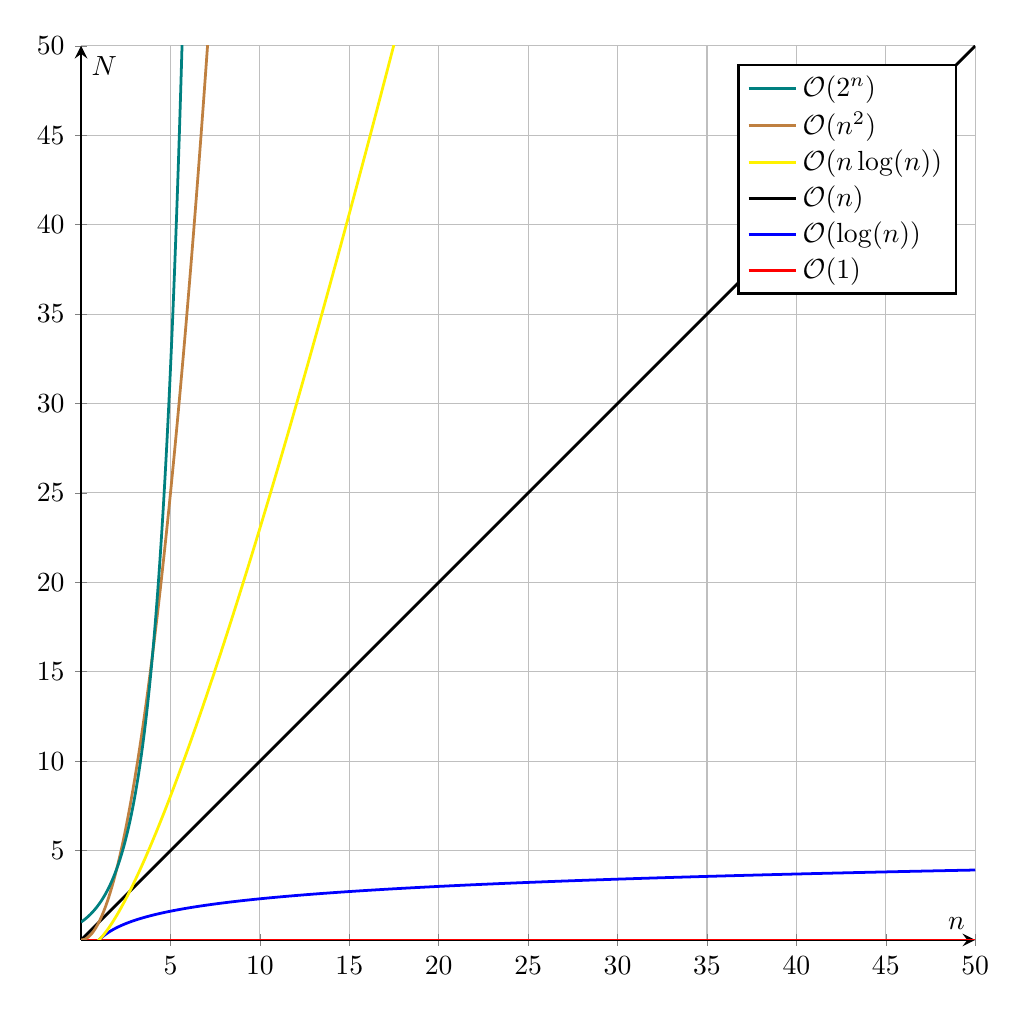
\begin{tikzpicture}[scale=1]
        \begin{axis}[
                width=15cm,
                unit vector ratio*=1 1,
                axis lines = middle,
                grid=major,
                ymin=0,
                ymax=50,
                xmin=0,
                xmax=50,
                xlabel = $n$,
                ylabel = $N$,
                xtick distance={5},
                ytick distance={5},
                disabledatascaling,
                cycle list name=color list,
                samples=250,
                solid,
                smooth,
                line width=1.0pt,
                no markers,
                legend cell align={left},
                reverse legend,
            ]

            \addplot +[domain=0:50]{0};         \addlegendentry{$\mathcal{O}(1)$};
            \addplot +[domain=0:50]{ln(x)};     \addlegendentry{$\mathcal{O}(\log(n))$};
                \addplot +[domain=0:50]{x};         \addlegendentry{$\mathcal{O}(n)$};
                \addplot +[domain=0:50]{x * ln(x)}; \addlegendentry{$\mathcal{O}(n \log(n))$};
            \addplot +[domain=0:50]{x^2};       \addlegendentry{$\mathcal{O}(n^2)$};
            \addplot +[domain=0:10]{2^x};        \addlegendentry{$\mathcal{O}(2^n)$};
        \end{axis}
    \end{tikzpicture}
\end{example}

\begin{example}[Komplexität]{Matrixmultiplikation}
    Problemgröße: $n$, ges.: $f(n)$ Anzahl der Rechen-Operationen in Abhängigkeit von der Matrix-Größe\\
    Notwendige Rechenzeit ist dann z.B.:
    \[T(n)=a\cdot f(n) + t_b\]
    mit $a$: Rechenzeit für eine Rechen- (Gleitkomma-) Operation,\\
    $b$: Rechenzeit für die Initialisierung und Beendigung des Algorithmus\\
    Formale Matrixmultiplikation:
    \[c_{i, j} = \sum\limits_{k=1}^{n}a_{i, k}\cdot b_{k, j}\]
    Bestimmung von $f(n)$: für jedes Element von $c$ sind $n$ Multiplikationen und $n-1$ Additionen durchzuführen.
    Also ergibt sich bei $n^2$ Elementen von $c$:
    \[f(n)=2\cdot n^3 - n^2\]

    TODO: Wording, Anschaulichkeit
\end{example}

\begin{bonus}{Master-Theorem}
    TODO
\end{bonus}

\begin{example}[Komplexität]{Strassen-Winograd}
    Effiziente Matrixmultiplikation:
    \begin{itemize}
        \item Matrizen werden in je vier Teilmatrizen der Größe $\frac{n}{2} \times \frac{n}{2}$ zerlegt:
              \begin{align*}
                  \begin{pmatrix}
                      A_{11} & A_{12} \\
                      A_{21} & A_{22}
                  \end{pmatrix}
                  \cdot
                  \begin{pmatrix}
                      B_{11} & B_{12} \\
                      B_{21} & B_{22}
                  \end{pmatrix}
                  =
                  \begin{pmatrix}
                      C_{11} & C_{12} \\
                      C_{21} & C_{22}
                  \end{pmatrix}
              \end{align*}
        \item Zusätzlich werden sieben neue Matrizen definiert:
              \begin{itemize}
                  \item $M_1 = (A_{12} - A_{22})\cdot(B_{21} + B_{22})$,
                  \item $M_2 = (A_{11} + A_{22})\cdot(B_{11} + B_{22})$,
                  \item $M_3 = (A_{11} - A_{21})\cdot(B_{11} + B_{12})$,
                  \item $M_4 = (A_{11} + A_{12})\cdot B_{22}$,
                  \item $M_5 = A_{11}\cdot(B_{21} - B_{22})$,
                  \item $M_6 = A_{22}\cdot(B_{21} - B_{11})$,
                  \item $M_7 = (A_{21} - A_{22})\cdot B_{11}$
              \end{itemize}
        \item Die vier Teilmatrizen der Ergebnismatrix ergeben sich damit wie folgt:
              \begin{itemize}
                  \item $C_{11} = M_1 + M_2 - M_4 + M_6$
                  \item $C_{12} = M_4 + M_5$
                  \item $C_{21} = M_6 + M_7$
                  \item $C_{22} = M_2 - M_3 + M_5 - M_7$
              \end{itemize}
    \end{itemize}
    Komplexität: $O(n^{\log_2 7})\approx O(n^2.807)$

\begin{defi}{Landau-Notation}
    Edmund Landau hat mit dem $O$-Symbol eine Notation geliefert,
    die den bestimmenden Term einer Funktion bezeichnet. \\
    $O(g(n))$ bezeichnet eine Klasse von Funktionen, wobei
    \[f(n) \in O(g(n))\]
    bedeutet, dass $f(n)$ höchstens so schnell wächst wie $g(n)$,
    das heißt, es gibt zwei positive Konstanten $c$ und $n_0$,
    für die gilt:
    \[|f(n)| \leq c \cdot |g(n)| \forall n \geq n_0\]
    (Definition hier nur für Funktionen über natürliche Zahlen)
\end{defi}

\begin{example}{Komplexitätsklassen}
    \begin{tabularx}{\textwidth}{|l|X|}
        \hline
        $O(1)$        & das Programm wird nur einmal linear durchlaufen, ohne von der Problemgröße abzuhängen (d.h. ohne Schleifen über $n$) $\to$ konstante Rechenzeit \\
        \hline
        $O(\log n)$   & z.B.\ bei Zerlegung von Problemen in Teilprobleme und Bearbeitung eines Teilproblems (binäre Suche)                                             \\
        \hline
        $O(n)$        & Algorithmen mit Schleifen $i = n_0 \ldots n$ (sequentielle Suche)                                                                               \\
        \hline
        $O(n \log n)$ & z.B.\ bei Zerlegung des Problems in Teilprobleme mit Bearbeitung aller Teilprobleme (Quicksort)                                                 \\
        \hline
        $O(n^2)$      & z.B.\ verschachtelte Schleifen (Paarweiser Vergleich)                                                                                           \\
        \hline
        $O(n^3)$      & z.B.\ dreifach verschachtelten Schleifen (Matrixmultiplikation)                                                                                 \\
        \hline
        $O(2n)$       & z.B.\ Suche in allen Kombinationen, Paaren oder Teilmengen                                                                                      \\
        \hline
    \end{tabularx}
\end{example}



